\documentclass[../Document.tex]{subfiles}
\graphicspath{{\subfix{../images/}}}

\begin{document}


\section{Chemistry}
\label{sec:intro/chemistry}
This section will detail different important notions in organic chemistry needed to understand the rest of this work.


%%% SubSection Chemical Notation %%%
\subsection{Chemical Notation}
Atoms are the building blocks of molecules and the bonds they can make are what allows the formation of complex structures. In organic chemistry, the atoms of interest are: Boron (B), Carbon (C), Nitrogen (N), Oxygen (O), Fluorine (F), Phosphorus (P), Sulphur (S), Chlorine (Cl), Bromine (Br) and Iodine (I).
The number of bonds an atom can make is limited by the electrons in its valence shell, also called valence electrons. This valence shell refers to the outermost layer of electrons.

A valence shell is made up of multiple subshells of different energy levels: 1s, 2s, 2p, 3s, 3p, 3d, etc. Each of these subshells can hold a different number of electrons and the valence shell of a given atom is said to be complete when the outermost subshells are full. This often comes back to reaching the configuration of a noble gas, which are the rightmost atoms in the periodic table.

Having a complete valence shell is the stable configuration that most atoms tend towards. To achieve this, atoms will make ionic bonds, a bond where an electron is taken from another atom, or covalent bonds, a bond where an electron is shared by two atoms. In the case of organic molecules, we will usually only consider covalent bonds.

If we take Hydrogen and Carbon as examples, two of the more common atoms in organic chemistry, they need one and four more electrons respectively to complete their valence shell. The earlier atoms used in organic chemistry have the following number of valence electrons: Boron has 3; Carbon has 4; Nitrogen and Sulfur have 5; Oxygen and Sulphur have 6; Fluorine, Chlorine, Bromine and Iodine have 7.
They can do this by making the corresponding number of covalent bonds required to complete their valence shell (commonly represented as line segments between atoms; see e.g. Figure~\ref{fig:complex_smiles}A).

\begin{figure}[t]
    \centering
    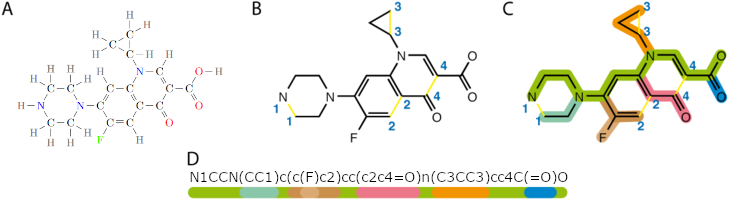
\includegraphics{images/complex_smiles.png}
    \caption[Deriving a SMILES representation for a molecule.]{Deriving a SMILES representation for a molecule (reproduced in part from \cite{wiki:complex-smiles}).
    The structural formula of the molecule (A), its skeletal formula stripped of all hydrogen atoms and with broken cycles (B), the selected main path (shown in green) and branches (C), and the corresponding SMILES notation (D).}
    \label{fig:complex_smiles}
\end{figure}

As seen in Figure~\ref{fig:complex_smiles}B, to reduce the visual clutter of molecular graphs, Carbon and Hydrogen atoms are omitted. Carbon atoms are simply vertices with no letter indicating anything and Hydrogen atoms are implicitly present to complete the valence shell of any atoms that appear to be missing a bond.


%%% SubSection Hydrogen Bonds %%%
\subsection{Hydrogen Bonds}
\label{subsec:intro/chem/hydrogen-bonds}
Hydrogen bonds are inter-molecular bonds caused by polarized molecules. They require a donor and an acceptor.
Covalent bonds do not always equally share the shared electron, specifically, the more electronegative an atom is, the more it pulls on the shared electron.
The electronegative atoms that interest us in the context of organic molecules are: Fluorine (F), Sulphur (S), O (Oxygen) and N (Nitrogen).

The \textbf{donor} is an electronegative atom linked to a Hydrogen atom. By pulling on the shared electron more than the Hydrogen atom does, the electronegative gains a partial negative charge. Inversely, the Hydrogen atom gains a partial positive charge. 

The \textbf{acceptor} is an electronegative atom with a free electron pair on its valence shell. This electron pair, can then attract the partially positively charged Hydrogen from the donor.

This attraction, between two different polarized molecules, is what we call a Hydrogen bond. The most famous example of this is in water and is the reason for many of water's interesting properties (cohesion, high boiling point, high heat capacity, surface tension, expands when frozen, etc). In this case, the Oxygen atom is both the donor and the acceptor. The Oxygen atom, acting as the acceptor, is negatively charged and can attract the positively charged Hydrogen atoms from other water molecules. The same atom will donate its positively charged Hydrogen atoms to other Oxygen atoms.


%%% SubSection Molecule Encodings %%%
\subsection{Molecule Encodings}
\label{sec:molecule-encodings}
Molecules can be encoded in many different ways. Two common methods are representing molecules as graphs or as one-dimensional strings.
We will be using a one-dimensional encoding in our work to simplify the representation and potentially allow a combined model using \gls{nlp} models.
We will present different one-dimensional encodings used in the molecule discovery field.


\begin{table}[t]
    \centering
    \begin{tabular}{|c|p{5in}|}
        \hline
        Encoding & Representation \\
        \hline
        \acrshort{inchi} & InChI=1S/C17H18FN3O3/c18-13-7-11-14(8-15(13)20-5-3-19-4-6-20)21(10-1-2-10)9-12(16(11)22)17(23)24/h7-10,19H,1-6H2,(H,23,24)\\
        \hline
        \acrshort{smiles} & 
        % This is actual SMILES
        N1CCN(CC1)c(c(F)c2)cc(c2c4=O)n(C3CC3)cc4C(=O)O
        % This is kekulized SMILES, aromatic rings are explicit
        % N1CCN(CC1)C(C(F)=C2)=CC(=C2C4=O)N(C3CC3)C=C4C(=O)O 
        \\
        \hline
        canonical \acrshort{smiles} & O=C(O)c1cn(C2CC2)c2cc(N3CCNCC3)c(F)cc2c1=O\\
        \hline
        DeepSMILES & O=CO)ccnCCC3)))cccNCCNCC6))))))cF)cc6c\%10=O\\
        \hline
        \acrshort{selfies} & [N][C][C][N][Branch1][Branch1][C][C][Ring1][=Branch1][C][Branch1]
        [=Branch1][C][Branch1][C][F][=C][=C][C][=Branch1][=Branch1][=C]
        [Ring1][Ring2][C][=O][N][Branch1][=Branch1][C][C][C][Ring1][Ring1]
        [C][=C][Ring1][Branch2][C][=Branch1][C][=O][O]\\
        \hline
    \end{tabular}
    \caption[Different encodings of the molecule shown in Figure~\ref{fig:complex_smiles}]{Different encodings of the molecule shown in Figure~\ref{fig:complex_smiles}. DeepSMILES could not originally encode the \gls{smiles} string, we converted the molecule to canon \gls{smiles} for it to encode it correctly.}
    \label{tab:different_encodings}
\end{table}

\subsubsection{\acrshort{inchi}}
\gls{inchi} is a notation standard introduced by the \gls{iupac}~\cite{inchi_intro}. It provides a unique one-dimensional representation of the molecule. The encoding contains information on both the structure and certain properties of the molecule. This representation was not adopted by the automated molecule discovery research community because of its low readability by both humans and machines. Instead, it has become commonly used in indexing and searching tasks (\eg databases).

\subsubsection{\acrshort{smiles}}
\gls{smiles} is a one-dimensional string representation for molecular encoding~\cite{smiles_intro}. This encoding is much simpler than \gls{inchi}, only maintaining the structural information required to reconstruct the molecule. However, any lost information can be recovered using different techniques. Admittedly, the process can be difficult and time-intensive to guarantee accurate results.
\david{Get sources showing which ppl do this}

If we picture a molecule as a graph where every vertex is an atom, a \gls{smiles} string would be the order in which we explore a tree-representation of the graph using a \gls{dfs}.
Since \gls{smiles} is a \gls{dfs} over a tree, any cyles that were in the original graph would be lost. Thankfully, \gls{smiles} considers this by designating a specific token to represent broken cycle bonds. This prevents losing the cycles when we convert the graph into a tree. These tokens are represented by number tokens as seen in Figure~\ref{fig:complex_smiles}B and, later, in D.
Similarly, when we reach a branching path in the tree, one side is chosen as the main branch, which is shown in green in Figure~\ref{fig:complex_smiles}C, while the other side is written between parentheses to indicate that it is a branch.

A very common concept in organic chemistry is aromatic rings. These are usually 5 or 6 atoms in a ring, the ring bonds alternate between single and double bonds. Due to their frequency, the \gls{smiles} language has started using a shorthand for it by writing atoms in aromatic rings using lowercase letters. This allows us to omit the alternating single and double bonds during writing and makes aromatic rings much more visible when reading a molecule.
Kekulized \gls{smiles} keeps these bonds explicit, but non-kekulized \gls{smiles} is preferred.

This encoding has gained a lot of popularity in the automated molecule discovery research community due to its age and ease of readability. Since its introduction, it has become the most popular string representation in automated discovery.
However it comes with certain issues that we must address. Unlike \gls{inchi}, \gls{smiles} does not offer a unique encoding for each molecule. It is therefore possible to generate two different strings that describe the same molecule.
Another prominent issue is linked to \gls{smiles}' special tokens. By requiring an opening token, as is needed to describe cycles, branches and isotopes (which we did not describe), any string that does not have corresponding open and close tokens is syntactically invalid. 

\gilles{À déplacer là où tu parleras des limites de la ML}
This can be problematic in token-by-token generation if these rules are not hard constraints, which is the case in \gls{ml} techniques since they lack the ability to impose long-term structure.

\gls{smiles} also has no check on the valence shells of the atoms within it. 
For example a Carbon atom, which wants to make 4 bonds to complete its valence shell, could be placed in such a way that it has 6 bonds.

There are some ways to generate canonical \gls{smiles} strings (\ie unique for a given molecule), however no consensus has been reached on which method to use.

This is the encoding that we use during our work, mainly due to its popularity within the automated molecule discovery community, which allowed us to find documentation and tools that helped during the work. We will present two other molecule encodings that were introduced to resolve issues within \gls{smiles}, but they were not used due to their relatively new appearance and, consequently, to their smaller research community.


\subsubsection{DeepSMILES}
DeepSMILES was introduced to answer some of \gls{smiles}' shortcomings~\cite{deepsmiles_intro}. It changes how branches and cycles are represented so that only one token is required. Instead of representing cycles using numbers as tags, they instead use numbers to indicate the size of the cycle and place the number at the end of the cycle. Similarly, branches no longer require opening branch tokens, instead they place as many branch closing tokens as there are atoms in the described branch.

Unfortunately, DeepSMILES is not perfect and sometimes fails to encode a molecule correctly. The example molecule used in Figure~\ref{fig:complex_smiles} cannot be directly converted into DeepSMILES from its \gls{smiles} format. This is a big issue, since the encoding could fail based on which bond in a cycle we choose to break to convert the graph into a tree. However, this can be avoided by first converting the molecule to canonical \gls{smiles}. The molecule still has an encoding in DeepSMILES, as shown in Table~\ref{tab:different_encodings}.

\subsubsection{\acrshort{selfies}}
Similarly to DeepSMILES, \gls{selfies}~\cite{selfies_intro} was introduced specifically for \gls{ml} applications, its language having been designed to minimize syntax invalidity and simplify the structure for \gls{ml} models.

To resolve some of \gls{smiles}' syntax problems (\ie branch and cycle invalidity), it associates each token to a numeric value. It then overloads the tokens following cycle or branch tokens, replacing them by their numeric value. In the case of branches, they place the token at the start of the branch and the overloaded value tells us how many of the future tokens are a part of this branch. For cycles, the token is placed at the end of the cycle and the overloaded value indicates how many atoms back we have to go to find the start of the cycle.

Another important difference is that all tokens are described between square brackets to remove some ambiguity. In \gls{smiles}, the square brackets are omitted for common atoms to improve readability.


%%% SubSection Lipinski Rule of Five %%%
\subsection{Lipinski's Rule of Five}
\label{sec:lipinski-rules}
Lipinski's Rule of Five is a set of rules describing properties that orally administered drugs tend to respect. While there are only four rules, each rule contains a value that is a multiple of five, which is where the name comes from. 

The rules are as follows:
\begin{itemize}
    \item The molecular weight must not exceed 500 Daltons.
    \item There must not be more than 10 Hydrogen-bond acceptors.
    \item There must not be more than 5 Hydrogen-bond donors.
    \item The logP must not exceed 5.
\end{itemize}

\paragraph{The molecular weight} is the simplest property to understand. By limiting the weight of the molecule, we tend to avoid molecules that are too large. It is important to note that Daltons are on a one-to-one scale with g/mol, which is the more commonly used unit. 

\paragraph{Hydrogen-bond acceptors} as seen in section~\ref{subsec:intro/chem/hydrogen-bonds}, are electronegative atoms (\eg F, S, N, O) with a free electron pair on their valence shell to act as an acceptor for the Hydrogen-bond.

\paragraph{Hydrogen-bond donors}, as seen in section~\ref{subsec:intro/chem/hydrogen-bonds}, are electronegative atoms linked to a Hydrogen atom. This Hydrogen atom will allow the Hydrogen-bond with an acceptor.

\paragraph{The logP} is an evaluation of how lipophilic or hydrophobic a molecule is, \ie how easily the molecule dissolves in fats as opposed to water. This is relevant when trying to control how a drug is absorbed in the human body.


\end{document}